\documentclass[journal=jcp,manuscript=suppinfo]{achemso}
\setkeys{acs}{maxauthors=0,articletitle=true}

%%%%%%%%%%%%%%%%%%%%%%%%%%%%%%%%%%%%%%%%%%

\usepackage{achemso}
\usepackage{graphics}
\usepackage{amssymb,amsfonts}
\usepackage{graphicx}
\usepackage[table]{xcolor}
\usepackage{threeparttable}
\usepackage{multirow}
\usepackage{caption}
\usepackage{subcaption}
\usepackage{booktabs}
\usepackage{colortbl}
\usepackage{amsmath}
\usepackage{amsopn}
\usepackage{siunitx}
\usepackage{bm}
\usepackage{color}
\usepackage{array}
\usepackage{lscape}
\usepackage{mciteplus}
\usepackage[version=3]{mhchem}
\usepackage{ulem}
\usepackage{listings}
\usepackage{enumerate}
\usepackage{makecell}

\captionsetup{labelfont=bf}
\SectionNumbersOn
\renewcommand{\thefootnote}{\fnsymbol{footnote}}
\newlength{\wordwidth}

%%%%%%%%%%%%%%%%%%%%%%%%%%%%%%%%%%%%%%%%%%

\author{Janus J. Eriksen}
\email{janus.eriksen@bristol.ac.uk}
\affiliation{School of Chemistry, University of Bristol, Cantock's Close, Bristol BS8 1TS, United Kingdom}
%
\author{Tyler Anderson}
\affiliation{Laboratory of Atomic and Solid State Physics, Cornell University, Ithaca, New York 14853, USA}
\author{J. Emiliano Deustua}
\affiliation{Department of Chemistry, Michigan State University, East Lansing, MI 48824, USA}
\author{Khaldoon Ghanem}
\affiliation{Max-Planck-Institut f{\"u}r Festk{\"o}rperforschung, 70569 Stuttgart, Germany}
\author{Diptarka Hait}
\affiliation{Kenneth S. Pitzer Center for Theoretical Chemistry, Department of Chemistry, University of California, Berkeley, California 94720, USA}
\alsoaffiliation{Chemical Sciences Division, Lawrence Berkeley National Laboratory, Berkeley, California 94720, USA}
\author{Mark R. Hoffmann}
\affiliation{Chemistry Department, University of North Dakota, Grand Forks, ND 58202-9024, USA}
\author{Seunghoon Lee}
\affiliation{Division of Chemistry and Chemical Engineering, California Institute of Technology, Pasadena, California 91125, USA}
\author{Ilias Magoulas}
\affiliation{Department of Chemistry, Michigan State University, East Lansing, MI 48824, USA}
\author{Jun Shen}
\affiliation{Department of Chemistry, Michigan State University, East Lansing, MI 48824, USA}
\author{Enhua Xu}
\affiliation{Graduate School of Science, Technology, and Innovation, Kobe University, 1-1 Rokkodai-cho, Nada-ku, Kobe 657-8501, Japan}
\author{Yuan Yao}
\affiliation{Laboratory of Atomic and Solid State Physics, Cornell University, Ithaca, New York 14853, USA}
\author{Ning Zhang}
\affiliation{Beijing National Laboratory for Molecular Sciences, Institute of Theoretical and Computational Chemistry, College of Chemistry and Molecular Engineering, Peking University, Beijing 100871, China}
%
\author{Ali Alavi}
\email{a.alavi@fkf.mpg.de}
\affiliation{Max-Planck-Institut f{\"u}r Festk{\"o}rperforschung, 70569 Stuttgart, Germany}
\alsoaffiliation{Department of Chemistry, University of Cambridge, Cambridge CB2 1EW, United Kingdom}
\author{Garnet Kin-Lic Chan}
\email{gkc1000@gmail.com}
\affiliation{Division of Chemistry and Chemical Engineering, California Institute of Technology, Pasadena, California 91125, USA}
\author{Martin Head-Gordon}
\email{mhg@cchem.berkeley.edu}
\affiliation{Kenneth S. Pitzer Center for Theoretical Chemistry, Department of Chemistry, University of California, Berkeley, California 94720, USA}
\alsoaffiliation{Chemical Sciences Division, Lawrence Berkeley National Laboratory, Berkeley, California 94720, USA}
\author{Wenjian Liu}
\email{liuwj@sdu.edu.cn}
\affiliation{Qingdao Institute for Theoretical and Computational Sciences, Shandong University, Qingdao, Shandong 266237, China}
\author{Piotr Piecuch}
\email{piecuch@chemistry.msu.edu}
\affiliation{Department of Chemistry, Michigan State University, East Lansing, MI 48824, USA}
\alsoaffiliation{Department of Physics and Astronomy, Michigan State University, East Lansing, MI 48824, USA}
\author{Sandeep Sharma}
\email{sandeep.sharma@colorado.edu}
\affiliation{Department of Chemistry and Biochemistry, The University of Colorado at Boulder, Boulder, Colorado 80302, USA}
\author{Seiichiro L. Ten-no}
\email{tenno@garnet.kobe-u.ac.jp}
\affiliation{Graduate School of Science, Technology, and Innovation, Kobe University, 1-1 Rokkodai-cho, Nada-ku, Kobe 657-8501, Japan}
\author{Cyrus J. Umrigar}
\email{cyrusumrigar@gmail.com}
\affiliation{Laboratory of Atomic and Solid State Physics, Cornell University, Ithaca, New York 14853, USA}
\author{J{\"u}rgen Gauss}
\email{gauss@uni-mainz.de}
\affiliation{Department Chemie, Johannes Gutenberg-Universit{\"a}t Mainz, Duesbergweg 10-14, 55128 Mainz, Germany}

\renewcommand*\titlesize{\Large}
\renewcommand*\authorsize{\small}
\renewcommand*\affilsize{\footnotesize}
\renewcommand*\emailsize{\scriptsize}

%%%%%%%%%%%%%%%%%%%%%%%%%%%%%%%%%%%%%%%%%%

\title[TITLE]{The Ground State Electronic Energy of Benzene}

%%%%%%%%%%%%%%%%%%%%%%%%%%%%%%%%%%%%%%%%%%

\begin{document}
%

\newpage

\section{Geometry}

The geometry of benzene used in our study is the MP2/6-31G$^{\ast}$ optimized structure from Ref. \citenum{sauer_thiel_cc3_benchmark_jcp_2008}, cf. Table \ref{geometry_SI_table}. For reference, the nuclear repulsion and Hartree-Fock energies are $E_{\text{nuc}} = 203.15350971$ $E_{\text{H}}$ and $E_{\text{HF}} = -230.721819131$ $E_{\text{H}}$, respectively.
%
\begin{table}[ht]
\begin{center}
\caption{C$_6$H$_6$ (in \AA).}
\label{geometry_SI_table}
\begin{tabular}{c|rrr}
\toprule
\multicolumn{1}{c|}{Atom} & \multicolumn{1}{c}{$x$} & \multicolumn{1}{c}{{\textbf{$y$}}} & \multicolumn{1}{c}{{\textbf{$z$}}} \\
\midrule\midrule
C & $0.000000$ & $1.396792$ & $0.000000$ \\
C & $0.000000$ & $-1.396792$ & $0.000000$ \\
C & $1.209657$ & $0.698396$ & $0.000000$ \\
C & $-1.209657$ & $-0.698396$ & $0.000000$ \\
C & $-1.209657$ & $0.698396$ & $0.000000$ \\
C & $1.209657$ & $-0.698396$ & $0.000000$ \\
H & $0.000000$ & $2.484212$ & $0.000000$ \\
H & $2.151390$ & $1.242106$ & $0.000000$ \\
H & $-2.151390$ & $-1.242106$ & $0.000000$ \\
H & $-2.151390$ & $1.242106$ & $0.000000$ \\
H & $2.151390$ & $-1.242106$ & $0.000000$ \\
H & $0.000000$ & $-2.484212$ & $0.000000$ \\
\midrule
\end{tabular}
\vspace{-1.4cm}
\end{center}
\end{table}
%

\section{Main Results}

Table \ref{results_SI_table} summarizes the results in Fig. 1 of the main study. Methods are ordered by the final correlation energy.
%
\begin{table}[ht]
\begin{center}
\caption{Summary of Fig. 1 from the main study.}
\label{results_SI_table}
\begin{tabular}{l|r}
\toprule
\multicolumn{1}{c|}{Method} & \multicolumn{1}{c}{$\Delta E$/m$E_{\text{H}}$} \\
\midrule\midrule
ASCI & $-860.0$ \\
iCI & $-861.1$ \\
CCSDTQ & $-862.4$ \\
DMRG & $-862.8$ \\
FCCR & $-863.0$ \\
MBE-FCI & $-863.0$ \\
CAD-FCIQMC & $-863.4$ \\
AS-FCIQMC & $-863.7$ \\
SHCI & $-864.3$ \\
\midrule
\end{tabular}
\vspace{-1.4cm}
\end{center}
\end{table}
%

\section{MBE-FCI}

%
\begin{figure}[ht!]
\begin{center}
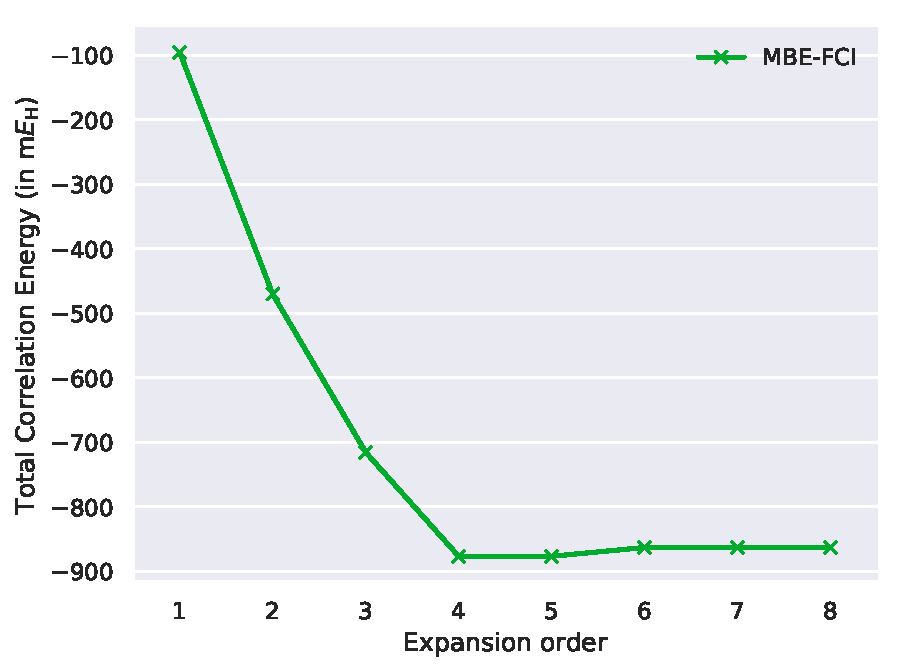
\includegraphics[scale=0.75]{figures/mbe_fci/mbe_fci.pdf}
\caption{MBE-FCI results.}
\label{mbe_fci_SI_fig}
\end{center}
\vspace{-0.6cm}
\end{figure}
%
In MBE-FCI theory~\cite{eriksen_mbe_fci_jpcl_2017,eriksen_mbe_fci_weak_corr_jctc_2018,eriksen_mbe_fci_strong_corr_jctc_2019,eriksen_mbe_fci_general_jpcl_2019}, the complete set of MOs for a given system is divided into a reference and an expansion space. An MBE-FCI expansion in the latter of these space hence recovers the residual correlation not captured by an FCI calculation constrained to the former. The MBE-FCI calculation of the present work is presented in Figure \ref{mbe_fci_SI_fig}, as performed in an embarrassingly parallel manner using the open-source {\texttt{PyMBE}} code~\cite{pymbe} on Intel Xeon E5-2697v4 (Broadwell) hardware (36 cores $@$ 2.3 GHz, 3.56 GB/core). The calculation was performed in a basis of localized Pipek-Mezey MOs~\cite{pipek_mezey_jcp_1989} with a ($6e$,$6$o) reference space consisting of the $\pi$- and $\pi^{\ast}$-orbitals and electrons. The final correlation energy is $\Delta E_{\text{MBE-FCI}} = -863.03$ m$E_{\text{H}}$.\\

In the course of preparing the code for running high-accuracy MBE-FCI calculations on the benzene molecule, a new screening protocol was implemented. At each order, MOs are screened away from the full expansion space according to their relative (absolute) magnitude, which in turn leads to a reduced number of increment calculations at the orders to follow. Specifically, only the MOs of the expansion space (at any given order) that give rise to the numerically largest increments will be retained at the following order. For the calculation of the present work, the percentages of the expansion space retained ($a_{\text{retain}}$) alongside the number of individual CASCI calculations at any given order ($K_{\text{CASCI}}$) are presented in Table \ref{mbe_fci_SI_table}. In addition, a number of optimizations were made to the code base. Most crucially, a new pruning scheme was introduced to make sure that only non-redundant increments are stored in memory throughout the total MBE-FCI calculation. For instance, once the $i$th MO gets screened away from the expansion space, all increments at lower orders, which reference this MO, are not needed anymore and may thus be pruned. This allows for significantly larger problem sizes to be treated by the method. As such, the limiting factor in converging MBE-FCI even tighter for the problem at hand, that is, screening less throughout the expansion, is related to available computer ressources rather than physical memory.
%
\begin{table}[ht]
\begin{center}
\caption{MBE-FCI calculation details.}
\label{mbe_fci_SI_table}
\begin{tabular}{l|r|r|r}
\toprule
\multicolumn{1}{c|}{Order} & \multicolumn{1}{c|}{$a_{\text{retain}}/\%$} & \multicolumn{1}{c|}{$\Delta E$/m$E_{\text{H}}$} & \multicolumn{1}{c}{$K_{\text{CASCI}}$} \\
\midrule\midrule
1 & 100.0 & $-95.1132$ & 102 \\
2 & 100.0 & $-469.884$ & 5,151 \\
3 & 100.0 & $-715.265$ & 171,700 \\
4 & 100.0 & $-876.637$ & 4,249,575 \\
5 & 100.0 & $-876.624$ & 83,291,670 \\
6 & 50.0 & $-862.988$ & 1,346,548,665 \\
7 & 25.0 & $-863.027$ & 115,775,100 \\
8 & 12.5 & $-863.027$ & 495 \\
\midrule
\end{tabular}
\vspace{-1.4cm}
\end{center}
\end{table}
%

\section{DMRG}

For details on DMRG theory, please see a number of contemporary reviews on the topic~\cite{chan_dmrg_2011,wouters_dmrg_2014,knecht_dmrg_2016}. All DMRG calculations were performed using the {\texttt{BLOCK}} code~\cite{chan_head_gordon_dmrg_jcp_2002,chan_dmrg_jcp_2004,chan_polyacetylenes_jcp_2008,sharma_chan_dmrg_2012,chan_dmrg_2015}, executed through the {\texttt{PySCF}} program~\cite{pyscf_prog,pyscf_paper,pyscf_arxiv_2020}, on Intel Xeon CPU E5-2680v4 (28-36 cores $@$ 2.4 GHz, 9.85 GB/core) and Gold 6130 (32 cores $@$ 2.1 GHz, 6.0 GB/core) nodes. DMRG yields two separate results: a variational upper bound and an extrapolated number based on different bond dimensions. The lowest variational correlation energy is $\Delta E_{\text{DMRG(var)}} = -859.5$ m$E_{\text{H}}$, while the extrapolated result (infinite bond dimension estimate) is $\Delta E_{\text{DMRG}(\infty)} = -862.8$ m$E_{\text{H}}$, cf. Figure \ref{dmrg_SI_fig}. The standard procedure for estimating error bars from the extrapolation is to report these as a fraction of the extrapolation distance. However, the resulting uncertainties may become unreasonably large. Here, the estimate ($1/5$ extrapolation distance error metric) is $0.7$ m$E_{\text{H}}$, not to be confused with the error of the fit (about $0.2$ m$E_{\text{H}}$).
%
\begin{figure}[ht!]
\begin{center}
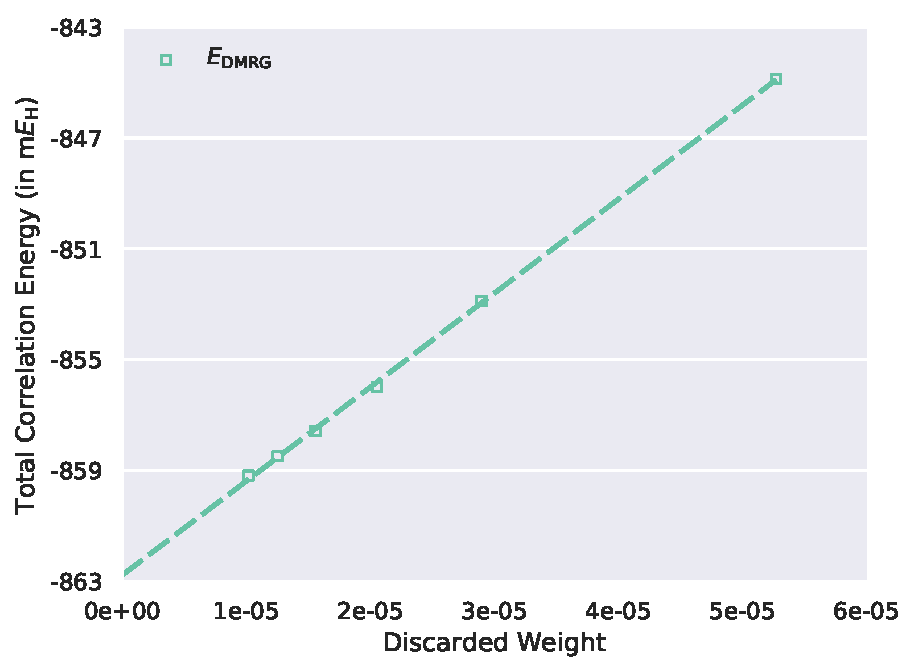
\includegraphics[scale=0.75]{figures/dmrg/dmrg.pdf}
\caption{DMRG results.}
\label{dmrg_SI_fig}
\end{center}
\end{figure}
%

\section{AS-FCIQMC}\label{as_fciqmc_SI_sect}

For details on the adaptive shift formalism, please see Ref. \citenum{ghanem_alavi_fciqmc_jcp_2019}. All AS-FCIQMC calculations were performed using the {\texttt{NECI}} code~\cite{neci} in parallel on Intel Xeon CPU E5-2698v4 nodes (40 cores $@$ 2.2 GHz, 6.4 GB/core). The orbitals used were those of a preceding RHF orbitals and the FCIQMC runs were performed in a basis of pure Slater determinants (no spin adaptation). Following an equilibration run with $\num{1.e8}$ walkers (yielding a correlation energy of $\Delta E_{\text{AS-FCIQMC(init)}} = -863.3\pm0.9$ m$E_{\text{H}}$), a first calculation with $\num{1.e9}$ (1B) walkers (growing from $\num{1.e8}$) yielded a correlation energy $\Delta E_{\text{AS-FCIQMC(1B)}} = -864.8\pm0.5$ m$E_{\text{H}}$. Next, a second calculation with $\num{2.e9}$ (2B) walkers (growing from $\num{1.e9}$) resulted in a correlation energy of $\Delta E_{\text{AS-FCIQMC(2B)}} = -863.7\pm0.3$ m$E_{\text{H}}$. The stochastic error bar of $0.3$ m$E_{\text{H}}$ is derived by averaging over the last 2637 time steps (discarding the first 5000 time steps for walker growth and equilibration period), and doing a blocking analysis. The AS‐FCIQMC(2B) result is used in Fig. 1 of the main study.

\section{CAD-FCIQMC}

A CAD-FCIQMC calculation consists of three steps~\cite{piecuch_monte_carlo_cc_prl_2017,piecuch_monte_carlo_cc_jcp_2018,piecuch_monte_carlo_eom_cc_jcp_2019,piecuch_mg_dimer_sci_adv_2020}: {\bf{(i)}} a stochastic FCIQMC run to produce the wave function for the subsequent cluster analysis (information only needed of the CI wave function through the $\{\bm{c}_4\}$ coefficients), {\bf{(ii)}} a cluster analysis of the wave function to extract CC cluster amplitudes through $\{\bm{t}_4\}$, and {\bf{(iii)}} a CCSD-like calculation in which $\{\bm{t}_1,\bm{t}_2\}$ are deterministically computed in the presence of $\{\bm{t}_3,\bm{t}_4\}$. In the context of the present work, the CAD-FCIQMC calculations were run on the AS-FCIQMC wave functions of Sect. \ref{as_fciqmc_SI_sect} (1B and 2B). Both the cluster analysis and the following CCSD-like calculation were performed using a specialized code developed in the Piecuch group on a shared-memory Dell node consisting of two 10-core Intel Xeon Silver 4114 (2.2 GHz, {\color{red}{XX}} GB/core) processors. The $\{\bm{t}_1,\bm{t}_2\}$ amplitudes extracted from the AS-FCIQMC wave function were used as an initial guess for the final CCSD-like iterations, and 10 iterations were needed to converge the final CAD-FCIQMC energy to within $\num{1.0e-6}$ $E_{\text{H}}$. To eliminate the need for storing large sets of the quadruples cluster amplitudes, the cluster analysis code used in this work stored only $\{\bm{t}_1,\bm{t}_2,\bm{t}_3\}$ amplitudes extracted from FCIQMC, while the $\{\bm{t}_4\}$ amplitudes were processed on the fly. Specifically, only the $\langle \Phi_{ij}^{ab} | (\hat{V}_N \hat{T}_4)_C | \Phi \rangle$ terms of the CCSD system (corrected for $\{\bm{t}_3,\bm{t}_4\}$) were stored, as the number of these scale as the number of doubly excited determinants ($| \Psi_{ij}^{ab} \rangle$) rather than the entire $\{\bm{t}_4\}$ vector.\\

%
\begin{table}[ht]
\begin{center}
\caption{CAD-FCIQMC calculation details.}
\label{cad_fciqmc_SI_table}
\begin{tabular}{l|r}
\toprule
\multicolumn{1}{c|}{Method} & \multicolumn{1}{c}{$\Delta E$/m$E_{\text{H}}$} \\
\midrule\midrule
AS-FCIQMC(1B) & $-864.8\pm0.5$ \\
CAD-FCIQMC-ext(1B) & $-867.01$ \\
CAD‐FCIQMC$[1$‐$5]$(1B) & $-864.09$ \\
CAD‐FCIQMC$[1,(3$+$4)/2]$(1B) & $-863.86$ \\
\hline
AS-FCIQMC(2B) & $-863.7\pm0.3$ \\
CAD-FCIQMC-ext(2B) & $-863.46$ \\
CAD‐FCIQMC$[1$‐$5]$(2B) & $-863.45$ \\
CAD‐FCIQMC$[1,(3$+$4)/2]$(2B) & $-863.44$ \\
CAD‐FCIQMC-ext(2B, 100-avg) & $-863.46$ \\
CAD‐FCIQMC$[1$‐$5]$(2B, 100-avg) & $-863.44$ \\
\midrule
\end{tabular}
\vspace{-0.6cm}
\end{center}
\end{table}
%
All CAD-FCIQMC results are presented in Table \ref{cad_fciqmc_SI_table}. To a first approximation (CAD-FCIQMC-ext), the correlation energy was computed using $\{\bm{t}_1,\bm{t}_2\}$ amplitudes extracted directly from the AS-FCIQMC wave function. Next, the final CAD-FCIQMC energy---obtained by solving for $\{\bm{t}_1\,\bm{t}_2\}$ in the presence of $\{\bm{t}_3,\bm{t}_4\}$---was computed in either of two ways, denoted as CAD‐FCIQMC$[1$‐$5]$ and CAD‐FCIQMC$[1,(3$+$4)/2]$. The information in the square brackets relates to the given treatment of the CCSD Goldstone-Hugenholtz diagrams quadratic in the $\hat{T}_2$ operator (adopting the diagram numbering from {\color{red}{Ref. ???}}); $[1$-$5]$ implies that all five of these are treated deterministically, while $[1,(3$+$4)/2]$ implies that this only applies to diagram 1 and an average of diagrams 3 and 4 (with the remaining contributions to the equation for the doubles amplitudes calculated using $\{\bm{t}_2\}$ amplitudes extracted directly from AS-FCIQMC). Further details on the CAD‐FCIQMC$[1,(3$+$4)/2]$ algorithm, which was originally considered in one of the approximate coupled-pair theories of {\color{red}{Ref. ???}} and recently implemented in the form of a DCSD approach to help capture strong correlations {\color{red}{(Ref. ???)}}, will be described in {\color{red}{Ref. ???}}. Finally, results are presented in Table \ref{cad_fciqmc_SI_table} for which the instantaneous AS-FCIQMC wave function---obtained at the end of a stochastic propagation---was replaced by an average over the last 100 time steps (100-avg). The CAD‐FCIQMC$[1$‐$5]$(2B) result is used in Fig. 1 of the main study.

\section{SHCI}

For details on the most recent version of SHCI theory, please see Ref. \citenum{li_sharma_umrigar_heat_bath_ci_jcp_2018}. All SHCI calculations were performed using the {\texttt{Arrow}} code~\cite{arrow} in parallel {\color{red}{on what hardware???}} ({\color{red}{XX}} cores $@$ {\color{red}{XX}} GHz, {\color{red}{XX}} GB/core). The computed SHCI results are presented in {\color{red}{Fig. \ref{shci_SI_fig} (Cyrus and Sandeep, can you please forward me information that would allow me to make a figure similar to Figs. \ref{asci_SI_fig} and \ref{ici_SI_fig}?)}}, and the final extrapolated correlation energy is estimated to be $\Delta E_{\text{SHCI}} = -864.3\pm1.5$ m$E_{\text{H}}$ with the error bar {\color{red}{derived how???}}.

\section{ASCI}
\label{sec:asci}
%
\begin{figure}[ht!]
\begin{center}
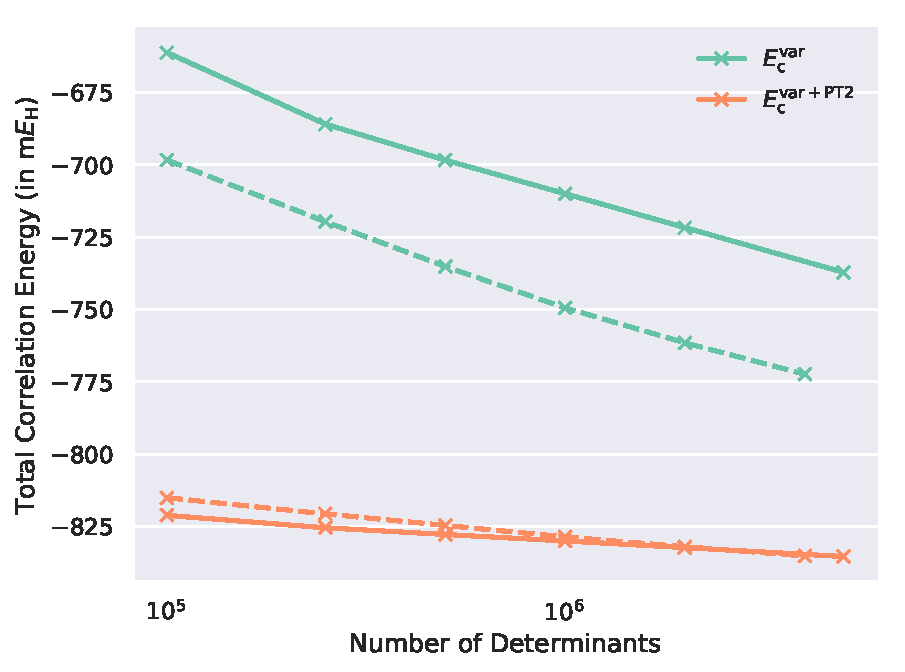
\includegraphics[scale=0.75]{figures/asci/asci.pdf}
\caption{ASCI results. Original results are plotted with solid lines, updated localized orbital results (not part of main study) are plotted with hashed lines.}
\label{asci_SI_fig}
\end{center}
\vspace{-0.6cm}
\end{figure}
%
Details on the most recent version of ASCI theory has recently been presented elsewhere~\cite{tubman_whaley_selected_ci_jctc_2020,tubman_whaley_selected_ci_pt_arxiv_2018}. 
All ASCI calculations were performed using a development version of Q-Chem 5.2\cite{shao2015advances}  on AMD EPYC 7401 hardware (2.0 GHz, 5.3 GB/core). The CI component was run in parallel over 24 processors but the subsequent Epstein-Nesbet PT2 correction was computed on a single processor. The active space orbitals were optimized from canonical HF MOs in an MCSCF manner (while only considering active-active rotations, i.e. keeping the core levels frozen), using $5\times 10^5$ ASCI selected determinants  \cite{levine2020casscf}, prior to PT2 calculations with varying number of determinants.
The computed ASCI results are presented in  Figure \ref{asci_SI_fig}, and the final extrapolated correlation energy is estimated to be $\Delta$E$_\textrm{ASCI}$ =-860.0 $\pm$ 0.2 m$E_{\text{H}}$ with the error bar spanned by the uncertainty in the extrapolation towards the limit of zero PT2 correction (standard deviation of a linear fit with last 3 points, as described in Ref \citenum{hait2019levels}).

\subsection{ASCI with localized orbitals}
\label{sec:asciloc}
Subsequent to the blind challenge, an additional effort was made to determine the impact of using spatial symmetry broken localized orbitals as an initial guess instead of delocalized canonical MOs. The occupied canonical orbitals were consequently Pipek-Mezey localized\cite{pipek1989fast} and the virtual space subjected to the Sano procedure\cite{sano2000elementary} to obtain the corresponding antibonding orbitals. These resulting orbitals were similarly optimized by active-active rotations in an MCSCF manner, using $5\times 10^5$ ASCI determinants\cite{levine2020casscf}. The optimized localized orbitals yielded significantly lower variational energies for a given size of ASCI wave function, although inclusion of PT2 resulted in values quite similar with those obtained from delocalized orbitals (as can be seen from Table \ref{tab:ascidata} and  Figure \ref{asci_SI_fig}). The lower magnitude of PT2 corrections nonetheless suggest that the localized orbital ASCI values are more reliable, especially with respect to extrapolation (by virtue of being closer to the $E_{PT2}\to 0$ limit). Extrapolation of the localized orbitals to the $E_{PT2}\to 0$ yields a correlation energy of -861.3$\pm$ 0.5 m$E_{\text{H}}$. 

It is however worth noting that this localized orbital result is essentially outside the range estimated from the original delocalized case (-860.0 $\pm$ 0.2 m$E_{\text{H}}$). This, in conjunction with the relatively low magnitude of correlation energy predicted by ASCI relative to other methods, indicates that the extrapolated ASCI error bar estimate is much too small in this case. This is likely a consequence of the stubbornly large $E_{PT2}$ values for the variational subspace sizes considered (as can be seen from Table \ref{tab:ascidata}), which likely prevents attainment of the asymptotic $E_{PT2}\to 0$ regime behavior for the extrapolation (despite $r^2$ of the linear fit being very close to 1, which is the origin of the too small error bars). It is however also worth noting that the extrapolation protocol nonetheless is quite effective, recovering $\sim$ -25/-26 m$E_{\text{H}}$ of the $\sim$ -28 m$E_{\text{H}}$ correlation not recovered by ASCI+PT2 alone (assuming an actual correlation energy of $\sim$ -863 m$E_{\text{H}}$). More reliable estimates from ASCI+PT2 would require larger variational subspaces than those studied in this work. Our original choice was partly determined by code limitations, though we considered $5\times 10^6$ determinants to be sufficient at the time of the blind challenge. 

\begin{table}[]
	\begin{tabular}{llll|llll}
		\multicolumn{4}{l}{Delocalized Orbitals (original blind test)} & \multicolumn{4}{l}{Localized orbitals}             \\\hline
		$N_\text{dets}$      & $E_{\mathrm{c}}^{\mathrm{var}}$    & $E_{\mathrm{c}}^{\mathrm{PT2}}$      & $E_{\mathrm{c}}^{\mathrm{var+PT2}}$    & $N_\text{dets}$    & $E_{\mathrm{c}}^{\mathrm{var}}$ & $E_{\mathrm{c}}^{\mathrm{PT2}}$   & $E_{\mathrm{c}}^{\mathrm{var+PT2}}$ \\
		$1\times10^5$  & -661.17        & -159.97    & -821.14            & $1\times10^5$ & -698.31     & -116.74 & -815.05         \\
		$2.5\times10^5$    & -685.91        & -139.54    & -825.45            & $2.5\times10^5$ & -719.63     & -101.03 & -820.65         \\
		$5\times10^5$    & -698.34        & -129.41    & -827.75            & $5\times10^5$ & -735.12     & -89.49  & -824.62         \\
		$1\times10^6$    & -709.96        & -120.04    & -830.00            & $1\times10^6$ & -749.43     & -79.17  & -828.60         \\
		$2\times10^6$    & -721.68        & -110.61    & -832.29            & $2\times10^6$ & -761.51     & -70.49  & -832.00         \\
		$5\times10^5$    & -737.13        & -98.25     & -835.38            & $4\times10^5$ & -772.35     & -62.83  & -835.18         \\\hline 
		Fit         &                &            & -860.0$\pm$0.2            & Fit      &             &         & -861.3$\pm$0.5       
	\end{tabular}
	\caption{Correlation energies  ($E_{\mathrm{c}}$, in m$E_{\text{H}}$) for ASCI wave functions with various number of determinants ($N_\text{dets}$).}
	\label{tab:ascidata}
\end{table}


%All ASCI calculations were performed using {\color{red}{what code???}} in parallel on AMD EPYC 7401 hardware (24 cores $@$ 2.0 GHz, {\color{red}{XX}} GB/core). The computed ASCI results are presented in Figure \ref{asci_SI_fig}, and the final extrapolated correlation energy is estimated to be $\Delta E_{\text{ASCI}} = -859.97\pm0.2$ m$E_{\text{H}}$ with the error bar spanned by the uncertainty in the extrapolation towards the limit of zero PT2 correction (standard deviation of a linear fit with last 3 points).

\section{iCI}

The iCI approach~\cite{liu_hoffmann_ici_jctc_2016,liu_hoffmann_ici_jctc_2020}, which was born from the restricted static-dynamic-static~\cite{liu_hoffmann_sds_tca_2014} (SDS) framework for treating strongly correlated electrons, is a method designed to converge from above to the FCI limit within just a few iterations, by constructing and diagonalizing a $3N_P\times3N_P$ Hamiltonian matrix at each macro/micro-iteration, even when starting with a very poor initial guess. Here, $N_P$ denotes the number of target states. This convergence behaviour is hardly surprising, since the lowest order realization of the SDS framework, i.e., SDSPT2~\cite{liu_hoffmann_sdspt2_mp_2017}, already performs very well for prototypical systems of variable near degeneracies. However, iCI is computationally very expensive. One way out is to combine iCI with the idea of configuration selection, so as to generate a compact variational space for static correlation. The remaining dynamic correlation is treated via Epstein-Nesbet PT2. In brief, iCI has the following features: {\bf{(i)}} Full spin symmetry is always maintained by taking configuration state functions (CSF) as the many-electron basis. {\bf{(ii)}} Although the selection is performed on individual CSFs, it is orbital configurations (oCFG) that are used as the organizing units. {\bf{(iii)}} Given a coefficient pruning threshold, $C_{\text{min}}$ (which determines the size of the variational space for static correlation), the selection of important oCFGs/CSFs is performed iteratively until convergence. {\bf{(iv)}} At each iteration in the growth of the wave function, the first-order interacting space is decomposed into disjoint subspaces, so as to reduce memory requirement on one hand and facilitate parallelization on the other. {\bf{(v)}} Upper bounds (which involve only two-electron integrals) for the interactions between doubly connected oCFG pairs are used to screen each first-order interacting subspace before the first-order coefficients of individual CSFs are evaluated. {\bf{(vi)}} The diagonalization of the Hamiltonian matrix in the variational space is achieved by the iterative vector interaction (iVI) method\cite{iVIa,iVIb} (which, for $N_p$ roots, constructs and diagonalizes a $3N_p\times 3N_p$ matrix in each iteration). {\bf{(vii)}} Upon termination of the selection, dynamic correlation is estimated by using state-specific Epstein-Nesbet PT2 (iCIPT2). Results were obtained in $D_{2\text{h}}$ point group symmetry using either HF or natural (NO) orbitals, cf. Fig. \ref{ici_SI_fig}, of which the linearly extrapolated (using the last six data points) iCIPT2(NO) result of $\Delta E_{\text{iCIPT2(NO)}} = -861.05\pm0.5$ m$E_{\text{H}}$ is used in Fig. 1 of the main study, cf. Table \ref{OldNO} and Fig. \ref{BenzeneEn}. Calculations were run using BDF (Beijing Density Functional) program~\cite{bdf_prog_tca_1997,bdf_prog_jcp_2020} on a single node with two Intel Xeon E5-2640 v3 processors (16 cores $@$ 2.6 GHz, 8.0 GB/core), and the OpenMP efficiency was approximately $50$ $\%$.\\

%
\begin{figure}[ht!]
\begin{center}
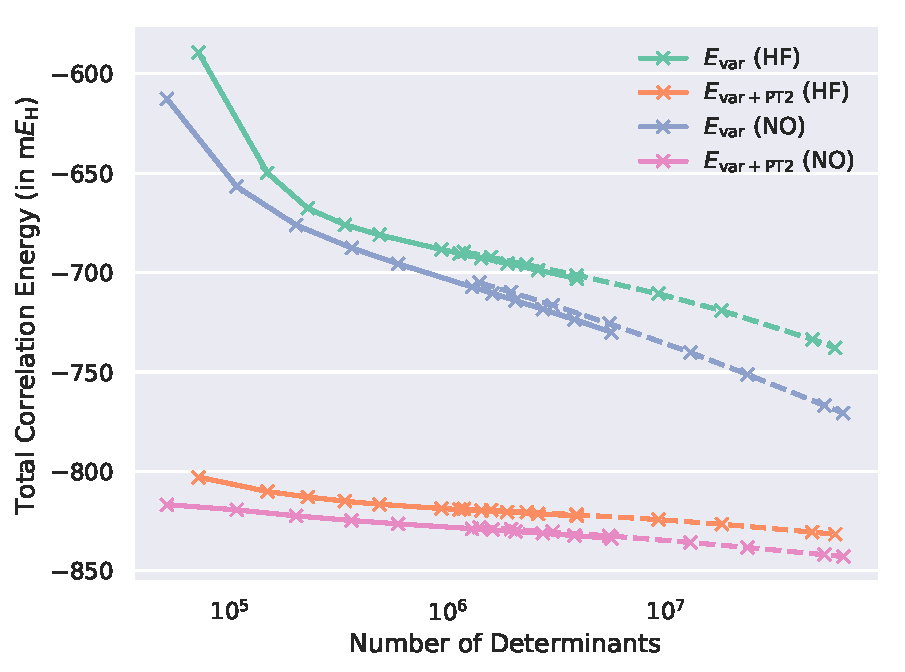
\includegraphics[scale=0.75]{figures/ici/ici.pdf}
\caption{iCI results. Original results are plotted with solid lines, updated results (not part of main study) are plotted with hashed lines.}
\label{ici_SI_fig}
\end{center}
\vspace{-0.6cm}
\end{figure}
%
Following the submission of the iCI result in Fig. 1 of the main study (Ref. \citenum{liu_hoffmann_ici_jctc_2020}), the efficiency of the method was increased by a factor of nearly 20. As such, the same $C_{\text{min}}$ values now always lead to smaller variational space, which has allowed for larger calculations than what was previously possible using either canonical HF orbitals or NOs. These updated results (not part of the blind challenge) are also presented in Fig. \ref{ici_SI_fig} (with hashed lines), cf. also Table \ref{NewNO} and Fig. \ref{BenzeneEnNew}. These are estimated to be more accurate than the original results since the selected variational space is larger. Moreover, the updated iCIPT2(NO) results are again estimated to be more reliable than the corresponding iCIPT2(HF) results since the former are always lower than the latter for each considered $C_{\text{min}}$ value. Furthermore, the gap between the smallest $C_{\text{min}}$ value and the extrapolated value is smaller for iCIPT2(NO) than for iCIPT2(HF). The linear extrapolations (again not shown) yield final correlation energies of $\Delta E_{\text{iCIPT2(HF,new)}} = -866.07\pm1.0$ m$E_{\text{H}}$ and $\Delta E_{\text{iCIPT2(NO,new)}} = -864.15\pm0.6$ m$E_{\text{H}}$.\\

For both the original and the updated results, the remaining difference between HF- and NO-based iCIPT2 (ca. 2 m$E_{\text{H}}$) may be understood in terms of space dimensions, as the cumulative effect of the unsampled CSFs remains substantial. To verify this argument, Cr$_2$/AVDZ may be used as an example. The difference between iCIPT2(HF) and iCIPT2(NO) in this case is within $0.1$ m$E_{\text{H}}$, correlating with the fact that the sampled space of CSFs makes up a considerably larger part of the FCI Hilbert space.

\begin{table}[!htp]
	\small
\caption{iCIPT2 blind-test correlation energies for benzene with natural orbitals }
	\begin{threeparttable}
		\centering
	\begin{tabular}{c|rrrrrrr}\toprule
		C$_{\text{min}}$&$N_{\mathrm{cfg}}$&$\tilde{N}_{\mathrm{csf}}$\tnote{a}&$\tilde{N}_{\mathrm{det}}$\tnote{b}
%		&$N_{csf,Q}$\tnote{c}
		&$E_{\mathrm{c}}^{\mathrm{var}}/\mathrm{mE_h}$&$E_{\mathrm{c}}^{\mathrm{PT2}}/\mathrm{mE_h}$&$E_{\mathrm{c}}/\mathrm{mE_h}$&$T/s$\tnote{c}\\\toprule
			$1.0\times10^{-3}$ &    14496 &    17890 &  50944&  -612.591  &  -204.133&  -816.724 &379\\
			$5.0\times10^{-4}$ &    28188 &    36448 & 106317&  -656.729  &  -162.637&  -819.366 &669\\
			$3.0\times10^{-4}$ &    48373 &    65080 & 199486&  -676.147  &  -146.237&  -822.384 &1481\\
			$2.0\times10^{-4}$ &    78947 &   109831 & 358274&  -687.627  &  -137.072&  -824.699 &2794\\
			$1.5\times10^{-4}$ &   119580 &   170356 & 586272&  -695.623  &  -130.780&  -826.403 &5066\\
			$1.0\times10^{-4}$ &   234640 &   344959 &1277001&  -707.243  &  -121.564&  -828.807 &15206\\
			$9.0\times10^{-5}$ &   284068 &   421316 &1585683&  -710.440  &  -119.020&  -829.460 &22335\\
			$8.0\times10^{-5}$ &   353743 &   529909 &2028558&  -714.110  &  -116.113&  -830.223 &38399\\
			$7.0\times10^{-5}$ &   456337 &   692215 &2697171&  -718.441  &  -112.694&  -831.135 &49238\\
			$6.0\times10^{-5}$ &   615593 &   947846 &3759324&  -723.616  &  -108.673&  -832.289 &77344\\
			$5.0\times10^{-5}$ &   878837 &  1381837 &5580152&  -729.983  &  -103.707&  -833.690 &133551\\\midrule
			0.0\tnote{b}&&&&&&\multicolumn{2}{c}{-861.05$\pm$0.51}\\\bottomrule
		\end{tabular}
\begin{tablenotes}
\item[a]Number of selected CSFs.
\item[b]Estimated number of determinants according to the expression $\sum_I\frac{\tilde{N}_{\mathrm{csf}}^I}{N_{\mathrm{csf}}^I}N_{\mathrm{det}}^I$, with $N_{\mathrm{det}}^I$, $N_{\mathrm{csf}}^I$ and $\tilde{N}_{\mathrm{csf}}^I$ being the numbers of determinants, CSFs and selected CSFs of orbital configuration (oCFG) $I$, respectively.
\item[c](1) CPU: Intel(R) Xeon(R) E5--2640 v3$\times$2, 16 cores; (2) memory: 128 Gb;
			(3) parallelization: OpenMP, 16 threads.
\item[d]Linearly extrapolated result using values of the 9 smallest $C_{min}$. The error bar refers to the half length of 95\% confidence interval.
		\end{tablenotes}
	\end{threeparttable}
	\label{OldNO}
\end{table}

\begin{table}[!htp]
	\small
	\caption{iCIPT2 blind-test correlation energies for benzene with Hartree-Fock orbitals }
	\begin{threeparttable}
		\centering
	\begin{tabular}{c|rrrrrrr}\toprule
		C$_{\text{min}}$&$N_{\mathrm{cfg}}$&$\tilde{N}_{\mathrm{csf}}$\tnote{a}&$\tilde{N}_{\mathrm{det}}$\tnote{b}
%		&$N_{csf,Q}$\tnote{c}
		&$E_{\mathrm{c}}^{\mathrm{var}}/\mathrm{mE_h}$&$E_{\mathrm{c}}^{\mathrm{PT2}}/\mathrm{mE_h}$&$E_{\mathrm{c}}/\mathrm{mE_h}$&$T/s$\tnote{c}\\\toprule
			$1.0\times10^{-3}$ &    19811 &    24862 &  71137&  -589.336  &  -213.573&  -802.909 &301  \\
			$5.0\times10^{-4}$ &    38400 &    51025 & 147228&  -649.922  &  -160.205&  -810.127 &837  \\
			$3.0\times10^{-4}$ &    54907 &    76712 & 225685&  -667.714  &  -145.170&  -812.884 &1309 \\
			$2.0\times10^{-4}$ &    75868 &   109263 & 333495&  -675.959  &  -139.038&  -814.997 &2363 \\
			$1.5\times10^{-4}$ &   103807 &   150972 & 480806&  -681.083  &  -135.481&  -816.564 &3036 \\
			$1.0\times10^{-4}$ &   180981 &   269149 & 921928&  -688.358  &  -130.306&  -818.664 &9875 \\
			$9.0\times10^{-5}$ &   214438 &   320658 &1120558&  -690.363  &  -128.831&  -819.194 &12712\\
			$8.0\times10^{-5}$ &   261828 &   394778 &1410356&  -692.695  &  -127.102&  -819.797 &17447\\
			$7.0\times10^{-5}$ &   331831 &   505250 &1849734&  -695.422  &  -125.065&  -820.487 &26334\\
			$6.0\times10^{-5}$ &   444010 &   683971 &2570589&  -698.767  &  -122.563&  -821.330 &42053\\
			$5.0\times10^{-5}$ &   640800 &  1001148 &3869123&  -703.066  &  -119.361&  -822.427 &72945\\\midrule
			0.0\tnote{b}&&&&&&\multicolumn{2}{c}{-863.32$\pm$0.54}\\\bottomrule
		\end{tabular}
\begin{tablenotes}
\item[a]Number of selected CSFs.
\item[b]Estimated number of determinants according to the expression $\sum_I\frac{\tilde{N}_{\mathrm{csf}}^I}{N_{\mathrm{csf}}^I}N_{\mathrm{det}}^I$, with $N_{\mathrm{det}}^I$, $N_{\mathrm{csf}}^I$ and $\tilde{N}_{\mathrm{csf}}^I$ being the numbers of determinants, CSFs and selected CSFs of orbital configuration (oCFG) $I$, respectively.
\item[c](1) CPU: Intel(R) Xeon(R) E5--2640 v3$\times$2, 16 cores; (2) memory: 128 Gb;
			(3) parallelization: OpenMP, 16 threads.
\item[d]Linearly extrapolated result using values of the 6 smallest $C_{min}$. The error bar refers to the half length of 95\% confidence interval.
		\end{tablenotes}
	\end{threeparttable}
	\label{OldHF}
\end{table}

\begin{figure}[!htp]
	\centering
	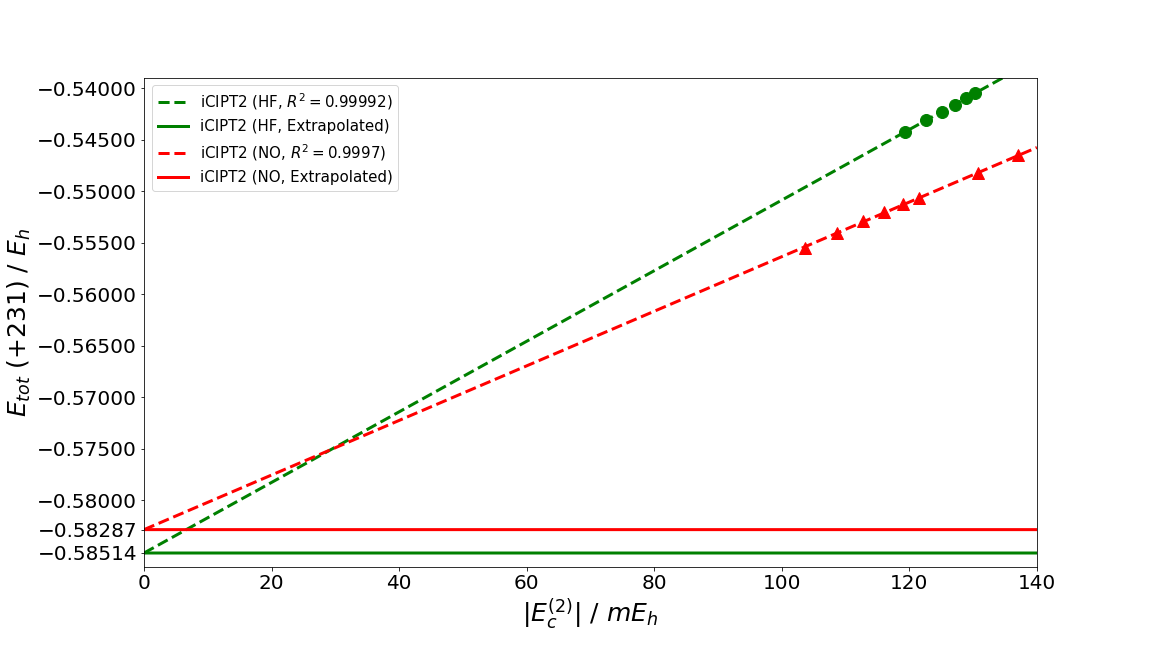
\includegraphics[width=\textwidth]{figures/ici/benzene_ici.png}
	\caption{ Linear fit of the correlation energy of benzene (blind test).}\label{BenzeneEn}
\end{figure}

\begin{table}[!htp]
	\small
	\caption{iCIPT2 correlation energies for benzene with natural orbitals (updated results).}
\begin{threeparttable}
	\centering
	\begin{tabular}{c|rrrrrrr}\toprule
		C$_{\text{min}}$&$N_{\mathrm{cfg}}$&$\tilde{N}_{\mathrm{csf}}$\tnote{a}&$\tilde{N}_{\mathrm{det}}$\tnote{b}
%		&$N_{csf,Q}$\tnote{c}
		&$E_{\mathrm{c}}^{\mathrm{var}}/\mathrm{mE_h}$&$E_{\mathrm{c}}^{\mathrm{PT2}}/\mathrm{mE_h}$&$E_{\mathrm{c}}/\mathrm{mE_h}$&$T/s$\tnote{c}\\\toprule
		$6.0\times10^{-5}$ &   245224 &   379662 & 1379097
%		& 2.74$\times10^{11}$
		&  -705.099  &  -122.996&  -828.095 &491\\
		$5.0\times10^{-5}$ &   330089 &   518448 & 1932040
%		& 4.00$\times10^{11}$
		&  -709.899  &  -119.182&  -829.081 &670\\
		$4.0\times10^{-5}$ &   486177 &   778940 & 2991370
%		& 6.42$\times10^{11}$
		&  -716.354  &  -114.087&  -830.441 &1039\\
		$3.0\times10^{-5}$ &   830917 &  1369463 & 5436028
%		& 1.17$\times10^{12}$
		&  -725.650  &  -106.817&  -832.467 &1834\\
		$2.0\times10^{-5}$ &  1809463 &  3121693 &12849733
%		& 2.65$\times10^{12}$
		&  -740.245  &  - 95.513&  -835.758 &4273\\
		$1.5\times10^{-5}$ &  3134922 &  5595481 &23479710
%		& 4.52$\times10^{12}$
		&  -751.271  &  - 87.026&  -838.298 &7597\\
		$1.0\times10^{-5}$ &  6555147 & 12315752 &52744912
%		& 8.88$\times10^{12}$
		&  -766.783  &  - 75.134&  -841.918 &19299\\
		$9.0\times10^{-6}$ &  7869797 & 14995161 &64497488
%		& 1.04$\times10^{13}$
		&  -770.695  &  - 72.139&  -842.834 &33344\\\midrule
		0.0\tnote{d}&&&&&&\multicolumn{2}{c}{-864.15$\pm$0.57}\\\bottomrule
	\end{tabular}
\begin{tablenotes}
	\item[a]Number of selected CSFs.
	\item[b]Estimated number of determinants according to the expression $\sum_I\frac{\tilde{N}_{\mathrm{csf}}^I}{N_{\mathrm{csf}}^I}N_{\mathrm{det}}^I$, with $N_{\mathrm{det}}^I$, $N_{\mathrm{csf}}^I$ and $\tilde{N}_{\mathrm{csf}}^I$ being the numbers of determinants, CSFs and selected CSFs of orbital configuration (oCFG) $I$, respectively.
%	\item[c]Number of CSFs in Q space.
	\item[c](1) CPU: Intel(R) Xeon(R) Gold 6240 $\times$4, 72 cores; (2) memory: 768 Gb; (3) parallelization: OpenMP, 72 threads.
	\item[d]Linearly extrapolated result using values of the 6 smallest $C_{min}$. The error bar refers to the half length of 95\% confidence interval.
\end{tablenotes}
\end{threeparttable}
\label{NewNO}
\end{table}

\begin{table}[!htp]
	\small
	\caption{iCIPT2 correlation energies for benzene with Hartree-Fock orbitals (updated results).}
\begin{threeparttable}
	\begin{tabular}{c|rrrrrrr}\toprule
		C$_{\text{min}}$&$N_{\mathrm{cfg}}$&$\tilde{N}_{\mathrm{csf}}$\tnote{a}&$\tilde{N}_{\mathrm{det}}$\tnote{b}
%		&$N_{csf,Q}$\tnote{c}
		&$E_{\mathrm{c}}^{\mathrm{var}}/\mathrm{mE_h}$&$E_{\mathrm{c}}^{\mathrm{PT2}}/\mathrm{mE_h}$&$E_{\mathrm{c}}/\mathrm{mE_h}$&$T/s$\tnote{c}\\\toprule
	$6.0\times10^{-5}$ &  221314 &   338334 & 1172202
%	&  1.76$\times10^{11}$
	& -689.523 &    -129.322 &  -818.846 &326\\
	$5.0\times10^{-5}$ &  282405 &   439038 & 1561473
%	&  2.38$\times10^{11}$
	& -692.337 &    -127.201 &  -819.539 &426\\
	$4.0\times10^{-5}$ &  391414 &   620645 & 2273564
%	&  3.63$\times10^{11}$
	& -696.048 &    -124.424 &  -820.473 &621\\
	$3.0\times10^{-5}$ &  631646 &  1017094 & 3856238
%	&  6.86$\times10^{11}$
	& -701.315 &    -120.475 &  -821.790 &1109\\
	$2.0\times10^{-5}$ & 1398298 &  2301712 & 9150757
%	&  1.86$\times10^{12}$
	& -710.687 &    -113.578 &  -824.265 &2749\\
	$1.5\times10^{-5}$ & 2583842 &  4359388 &17861976
%	&  3.66$\times10^{12}$
	& -719.137 &    -107.437 &  -826.574 &5387\\
	$1.0\times10^{-5}$ & 6206395 & 10978445 &46457235
%	&  8.63$\times10^{12}$
	& -733.630 &    - 96.926 &  -830.557 &14470\\
	$9.0\times10^{-6}$ & 7736950 & 13878500 &59119837
%	&  1.05$\times10^{13}$
	& -737.772 &    - 93.920 &  -831.692 &20203\\\midrule
	0.0\tnote{b}&&&&&&\multicolumn{2}{c}{-866.07$\pm$0.99}\\\bottomrule
	\end{tabular}
\begin{tablenotes}
	\item[a]Number of selected CSFs.
	\item[b]Estimated number of determinants according to the expression $\sum_I\frac{\tilde{N}_{\mathrm{csf}}^I}{N_{\mathrm{csf}}^I}N_{\mathrm{det}}^I$, with $N_{\mathrm{det}}^I$, $N_{\mathrm{csf}}^I$ and $\tilde{N}_{\mathrm{csf}}^I$ being the numbers of determinants, CSFs and selected CSFs of orbital configuration (oCFG) $I$, respectively.
%	\item[c]Number of CSFs in Q space.
	\item[c](1) CPU: Intel(R) Xeon(R) Gold 6240 $\times$4, 72 cores; (2) memory: 768 Gb; (3) parallelization: OpenMP, 72 threads.
	\item[d]Linearly extrapolated result using values of the 6 smallest $C_{min}$. The error bar refers to the half length of 95\% confidence interval.
\end{tablenotes}
\end{threeparttable}
\label{NewHF}
\end{table}

\begin{figure}[!htp]
	\centering
	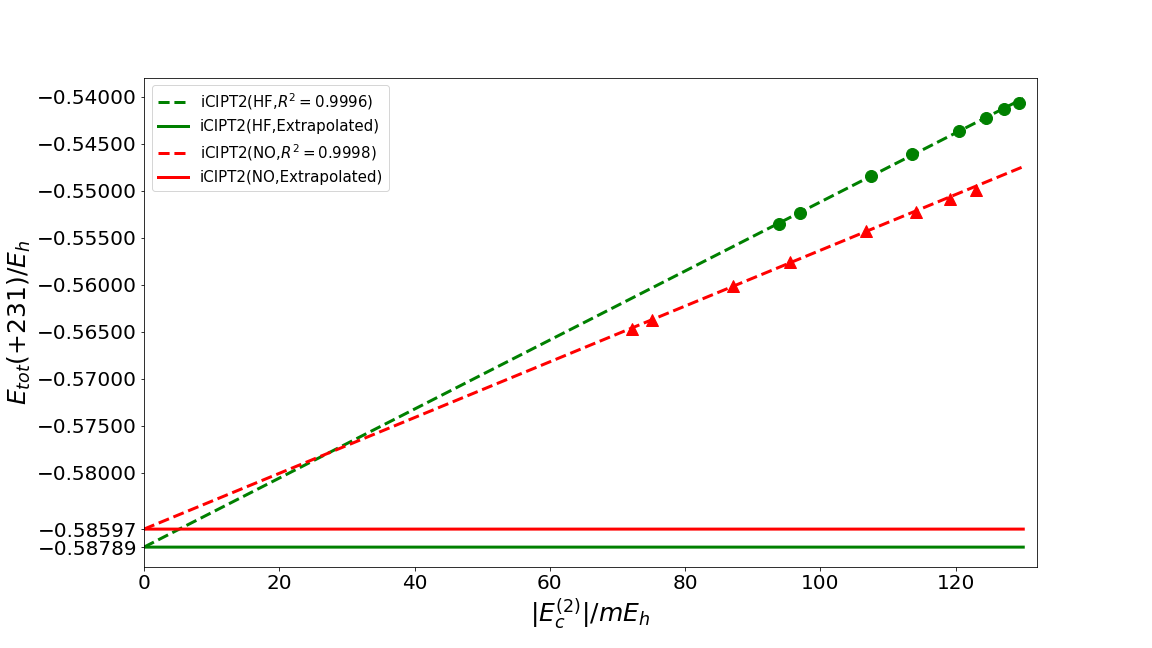
\includegraphics[width=\textwidth]{figures/ici/benzene_ici_updated.png}
	\caption{Linear fit of the correlation energy of benzene (updated results).}\label{BenzeneEnNew}
\end{figure}

\begin{table}[!htp]
	\centering
	\caption{Linearly extrapolated iCIPT2 correlation energies ($E_{\mathrm{c}}$ in $\mathrm{mE_h}$) for benzene and
extrapolation errors (in $\mathrm{mE_h}$). A: extrapolation distance; B: standard deviation; C:
half length of 95\% confidence interval.}
	\begin{tabular}{ccccccrc}\toprule
		&Orbitals
		&\makecell{$E_{\mathrm{c}}$}
		&\makecell{A}
		&\makecell{B}
		&\makecell{C}
		&CPU/h&memory/Gb
		\\\toprule
		\multirow{2}{*}{Blind Test}
		&NO&-861.05&27.36&0.22&0.51&1545&$\sim$650\\
		&HF&-863.32&40.89&0.19&0.54&836&$\sim$650\\\midrule
		\multirow{2}{*}{Updated}
		&NO&-864.15&21.32&0.21&0.57&1348&$\sim$610\\
		&HF&-866.07&34.38&0.36&0.99&891&$\sim$610\\\bottomrule
	\end{tabular}
\label{iCIsum}
\end{table}

\section{FCCR}

The size-extensive FCCR method exploits screenings within the single-reference CC formalism for constructing the excitation manifold $({\mathcal P})$ and to exclude insignificant operation mostly arising from the nonlinear terms of the working equation~\cite{ten_no_fcc_prl_2018}. The subsequent FCCR(2) computes the second-order perturbative correction to FCCR using the entire interacting space $({\mathcal Q})$ orthogonal to ${\mathcal P}$ generated through $[\hat H, \hat T_{\rm FCCR}]$~\cite{ten_no_fccr_2020}. For single-reference systems, FCCR(2') which approximate the $\hat \lambda$ amplitudes by $\hat T^{\dagger}$ is also available. All calculations were performed using the \texttt{GELLAN} program~\cite{gellan} in parallel on Intel Xeon Gold 6148 nodes (40 cores @ 2.4 GHz).\\

%
\begin{table}[ht!]
\begin{center}
\caption{FCCR calculation details (blind test).}
\label{fccr_SI_table}
\begin{tabular}{l|r}
\toprule
\multicolumn{1}{c|}{Method} & \multicolumn{1}{c}{$\Delta E$/m$E_{\text{H}}$} \\
\midrule\midrule
FCCR(MP) & $-860.1$ \\
FCCR(EN) & $-865.4$ \\
FCCR(avg) & $-862.8$ \\
FCCR(avg) + $\vartheta_{\mathcal O}$ corr. & $-863.0$ \\
\midrule
\end{tabular}
\vspace{-0.6cm}
\end{center}
\end{table}
%
Table \ref{fccr_SI_table} shows the result of FCCR(2') with the M{\o}ller-Plesset (MP) and Epstein-Nesbet (EN) partitionings with the connectivity threshold $\vartheta_{\mathcal C}=0.03$ and the operation threshold $\vartheta_{\mathcal O}=3.0 \times 10^{-7}$ as combined with the exclusion-principle-violating (EPV) form of the screening~\cite{ten_no_fcc_prl_2018}, leading to 4,818,644 FCCR cluster amplitudes. The FCI energy is estimated to lie very close to the average of the MP and EN results from various benchmarks (avg.), which may further be corrected for $\vartheta_{\mathcal O}$ based on CCSD, resulting in the estimate $-862.98 {\rm m}E_{\rm H}$. This calculation required 0.1M core hours invoking 640 MPI processes. The interacting space ${\mathcal Q}$ for the second-order correction is perfectly distributed to the processes, and the memory requirement of the present FCCR(2') calculation is at most 2GB per process.\\

%
\begin{table}[ht!]
\begin{center}
\caption{FCCR calculation details (updated results).}
\label{fccr_update_SI_table}
\begin{tabular}{r|r|r|r|r}
\toprule
\multicolumn{1}{c|}{$\vartheta_{\mathcal{P}}$} & \multicolumn{1}{c|}{$\Delta E$/m$E_{\text{H}}$} & \multicolumn{1}{c|}{$N_{\mathcal{P}}$} & \multicolumn{1}{c|}{$E^{(2)}$/m$E_{\text{H}}$} & \multicolumn{1}{c}{$N_{\mathcal{Q}}$} \\
\midrule\midrule
$5\times10^{-4}$   &  -849.05 & 109,860 & -81.09 & $2.2\times10^{8}$ \\
$4\times10^{-4}$   &  -852.25 & 137,421 & -62.36 & $2.6\times10^{8}$ \\
$3\times10^{-4}$   &  -854.93 & 174,914 & -46.71 & $3.7\times10^{8}$ \\
$2\times10^{-4}$   &  -856.84 & 229,842 & -35.11 & $6.4\times10^{8}$ \\
\hline
\multicolumn{1}{c|}{extrap.} &  -862.83 & \multicolumn{1}{c|}{---} & 0.0 & \multicolumn{1}{c|}{---} \\
\midrule
\end{tabular}
\vspace{-0.6cm}
\end{center}
\end{table}
%
A fast and more systematic estimate of the FCI limit is enabled by the extrapolation of FCCR(2). Table \ref{fccr_update_SI_table} presents an updated FCCR(2) correlation energy (not part of the blind challenge) along with the second-order correction of the MP partitioning as a function of the principal screening threshold $\vartheta\rm_{\mathcal P}$. Besides $\vartheta_{\mathcal O}$, the latest implementation of FCCR(2) controls the excitation manifold in terms of the two screening parameters, $\vartheta_{\mathcal P}$ to select the cluster operators of ${\mathcal P}$ perturbatively and $\vartheta_{\mathcal G}$ for the generator space $({\mathcal G})$ to discriminate strong correlation in ${\mathcal P}$.\cite{ten_no_fccr_2020} Except for $\vartheta_{\mathcal P}$, all screening parameters are fixed to be $\vartheta_{\mathcal G}=0.01$, $\vartheta_{\mathcal O}=10^{-7}$ for FCCR, and $\vartheta_{\mathcal O}=3.0\times10^{-6}$ for $E^{(2)}$. Tightening $\vartheta\rm_{\mathcal P}$ increases the accuracy of FCCR(2) according to the increasing dimensions of ${\mathcal P}$ and ${\mathcal Q}$. It is found that a linear relationship holds~\cite{ten_no_fccr_2020} between $\Delta E_{\rm FCCR(2)}$ and $E^{\rm (2)}$, as shown in Fig. \ref{fccr_updated_SI_fig}, and the best estimate of FCCR(2) based on the extrapolation is $-862.83{\rm m}E_{\rm H}$. The calculations for the four values of $\vartheta\rm_{\mathcal P}$ in Table \ref{fccr_update_SI_table} required 0.035M, 0.048M, 0.073M and 0.134M core hours, respectively, using 640 MPI processes. The algorithmic details of the FCCR(2) implementation and other applications will be elaborated in a separate paper~\cite{ten_no_fccr_2020}.
%
\begin{figure}[ht!]
\begin{center}
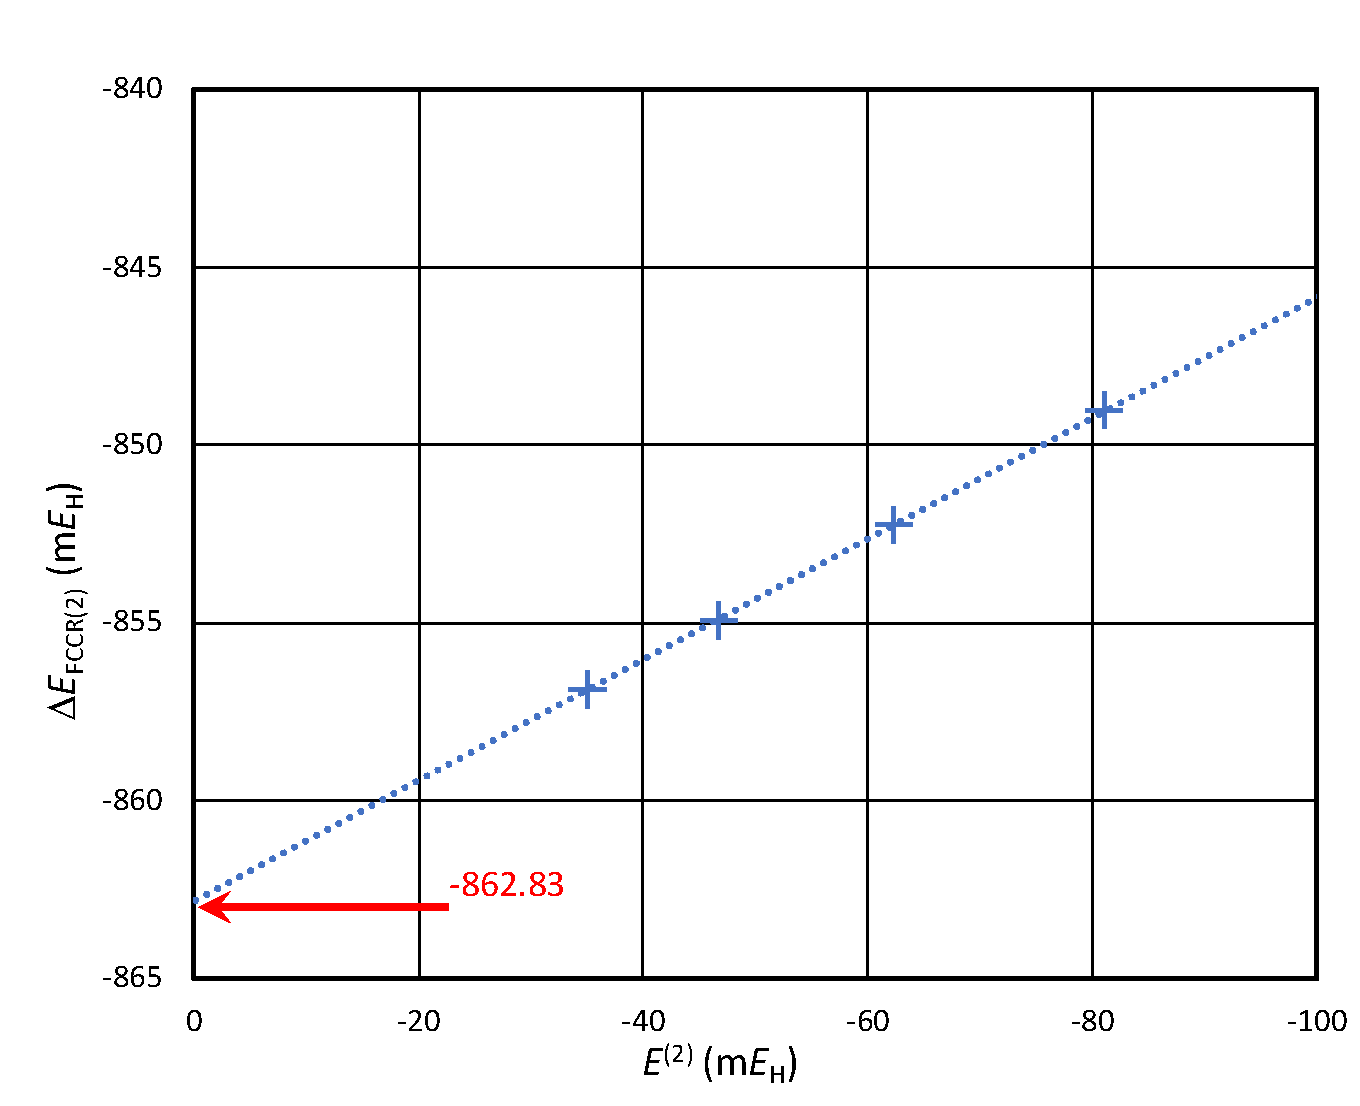
\includegraphics[scale=0.6]{figures/fccr/fccr.pdf}
\caption{Updated FCCR results. The linear extrapolation of the FCCR(2) energy.}
\label{fccr_updated_SI_fig}
\end{center}
\vspace{-0.6cm}
\end{figure}
%

\section{CCSDTQ}

The CCSDTQ~\cite{ccsdtq_paper_1_jcp_1991,ccsdtq_paper_2_jcp_1992} correlation energy of $\Delta E_{\text{CCSDTQ}} = -862.37$ m$E_{\text{H}}$ was obtained using the {\texttt{NCC}} module of the {\texttt{CFOUR}} program~\cite{matthews_stanton_ccsdtq_jcp_2015,ncc,cfour_paper,cfour} on a single Intel Xeon CPU E5-4620 node (8 cores $@$ 2.2 GHz, 15.0 GB/core). Convergence was reached in 10 iterations.

\section{Cluster Decomposition}

%
\begin{table}[ht!]
\begin{center}
\caption{Cluster decomposition ($L_2$-norm) of a 5M-determinant ASCI wave function (with delocalized orbitals) for excitation levels $1 \leq n \leq 6$.}
\label{cluster_decomp_SI_table}
\begin{tabular}{l|r|r|r}
\toprule
\multicolumn{1}{c|}{$n$} & \multicolumn{1}{c|}{$|\bm{c}_n|$} & \multicolumn{1}{c|}{$|\bm{t}_n|$} & \multicolumn{1}{c}{Ratio/$\%$} \\
\midrule\midrule
1 & $0.019477$ & $0.019477$ & $100.0$ \\
2 & $0.533103$ & $0.533108$ & $100.0$ \\
3 & $0.064742$ & $0.065137$ & $100.6$ \\
4 & $0.142888$ & $0.014178$ & $9.92$ \\
5 & $0.006201$ & $0.000465$ & $7.50$ \\
6 & $0.008792$ & $0.001948$ & $22.16$ \\
\midrule
\end{tabular}
\vspace{-0.6cm}
\end{center}
\end{table}
%
Table \ref{cluster_decomp_SI_table} presents results for a cluster decomposition~\cite{lehtola_head_gordon_fci_decomp_jcp_2017} of an ASCI wave function with $\num{5.e6}$ determinants (using delocalized orbitals, as described in Sec \ref{sec:asci}). These results indicate how most of the $\{\bm{c}_4\}$ (and higher order) CI coefficients comes from disconnected terms.  


Subsequent to the main study, a cluster decomposition was also carried out on a $\num{4.e6}$ determinant ASCI wave function with localized orbitals (as described in Sec \ref{sec:asciloc}), as this CI wave function had a lower variational energy than the previous one (-772 m$E_{\text{H}}$ correlation vs -737 m$E_{\text{H}}$) and was thus a better approximation to the true FCI wave function. The resulting values are provided in Table \ref{cluster_decomp_SI_table2}, which differ slightly from those in Table \ref{cluster_decomp_SI_table}. The general picture however remains the same, in that $\{\bm{c}_4\}$ and higher order excitations seem to mostly arise from disconnected terms. 

\begin{table}[ht!]
	\begin{center}
		\caption{Cluster decomposition ($L_2$-norm) of a 4M-determinant ASCI wave function (with localized orbitals) for excitation levels $1 \leq n \leq 6$.}
		\label{cluster_decomp_SI_table2}
		\begin{tabular}{l|r|r|r}
			\toprule
			\multicolumn{1}{c|}{$n$} & \multicolumn{1}{c|}{$|\bm{c}_n|$} & \multicolumn{1}{c|}{$|\bm{t}_n|$} & \multicolumn{1}{c}{Ratio/$\%$} \\
			\midrule\midrule
			1&	$0.01777$ &	$0.01777$&	$100.0$\\
			2&	$0.55063$ &	$0.55063$&	$100.0$\\
			3&	$0.06855$ &	$0.06868$&	$100.2$\\
			4&	$0.16486$ &	$0.01755$&	$10.65$\\
			5&	$0.00903$ &	$0.00076$&	$8.38$\\
			6&	$0.01610$ &	$0.00259$&	$16.11$\\
			\midrule
		\end{tabular}
		\vspace{-0.6cm}
	\end{center}
\end{table}


\newpage

\bibliography{si.bib}

%
\end{document}